\chapter{泛化}

本章将讨论理解和分析机器学习模型泛化能力的工具,即这些模型在未见过的测试样本上的表现。回想一下,对于监督学习问题,给定训练数据集 $\{(x^{(i)}, y^{(i)})\}_{i=1}^n$,通常通过最小化损失/成本函数 $J(\theta)$ 来学习模型 $h_\theta$,这鼓励 $h_\theta$ 拟合数据。例如,当损失函数是最小二乘损失(也称为均方误差)时,有 \(J(\theta) = \frac{1}{n} \sum_{i=1}^n \left(y^{(i)} - h_\theta(x^{(i)})\right)^2\) 这个用于训练的损失函数通常被称为\textbf{训练 (training)} 损失/误差/代价。

然而,最小化训练损失\textbf{并非}最终目标,它只是实现学习预测模型这一目标的途径。模型最重要的评估指标是在未见过的测试样本上的损失,通常被称为测试误差。形式上,从所谓的测试分布 $\mathcal{D}$ 中抽取一个测试样本 $(x, y)$,并衡量模型在其上的误差,例如均方误差 $(h_\theta(x) - y)^2$。测试样本随机性下的期望损失/误差称为测试损失/误差\footnote{在理论和统计文献中,通常将训练集 $\{(x^{(i)}, y^{(i)})\}_{i=1}^n$ 上的均匀分布称为经验分布,记为 $\mathcal{D}$,将总体分布称为 $\mathcal{D}$。因此(这是一部分原因),训练损失也称为经验损失/风险/误差,测试损失也称为总体损失/风险/误差。}。
\begin{equation}
    L(\theta) = \mathbb{E}_{(x,y) \sim \mathcal{D}}[(y - h_\theta(x))^2] \label{eq:8.1}
\end{equation}
请注意,误差的测量涉及计算期望,在实践中,可以通过对许多抽取的测试样本计算平均误差来近似,这些样本被称为测试数据集。这里训练集和测试集之间的关键区别在于测试样本是\textit{未见过的 (unseen)},因为训练过程没有使用这些测试样本。在经典的统计学习设置中,训练样本和测试样本都从与测试分布 $\mathcal{D}$ 相同的分布中抽取,但测试样本对于学习过程来说仍然是未见过的,而训练样本是已见过的\footnote{近年来,研究人员越来越关注“域偏移”的情况,即训练分布和测试分布不同。}。

由于训练集和测试集之间的这种关键区别,即使它们都从相同的分布 $\mathcal{D}$ 中抽取,测试误差也不一定总是接近训练误差\footnote{训练误差和测试误差之间的差异通常称为泛化差距。泛化误差在一些文献中指测试误差,在其他一些文献中指泛化差距。}。因此,成功最小化训练误差可能并不总是导致测试误差很小。如果模型在训练集上准确预测数据,但在其他测试样本上泛化能力不好,通常说模型\textbf{过拟合 (overfits)} 数据,即训练误差小而测试误差大。如果训练误差相对较大\footnote{例如,大于回归问题中数据的内在噪声水平。}(在这种情况下,测试误差通常也相对较大),则说模型\textbf{欠拟合 (underfits)} 数据。

本章研究学习过程如何影响测试误差,特别是模型参数化的选择。将测试误差分解为“偏差”和“方差”项,并研究模型参数化的选择及其权衡如何影响它们。利用偏差-方差权衡,将讨论何时发生过拟合和欠拟合以及如何避免。还将讨论 \ref{sec:8.2} 节中的双下降现象和 \ref{sec:8.3} 节中的一些经典理论结果。


\section{偏差-方差均衡}\label{sec:8.1}

\begin{figure}[H]
    \centering
    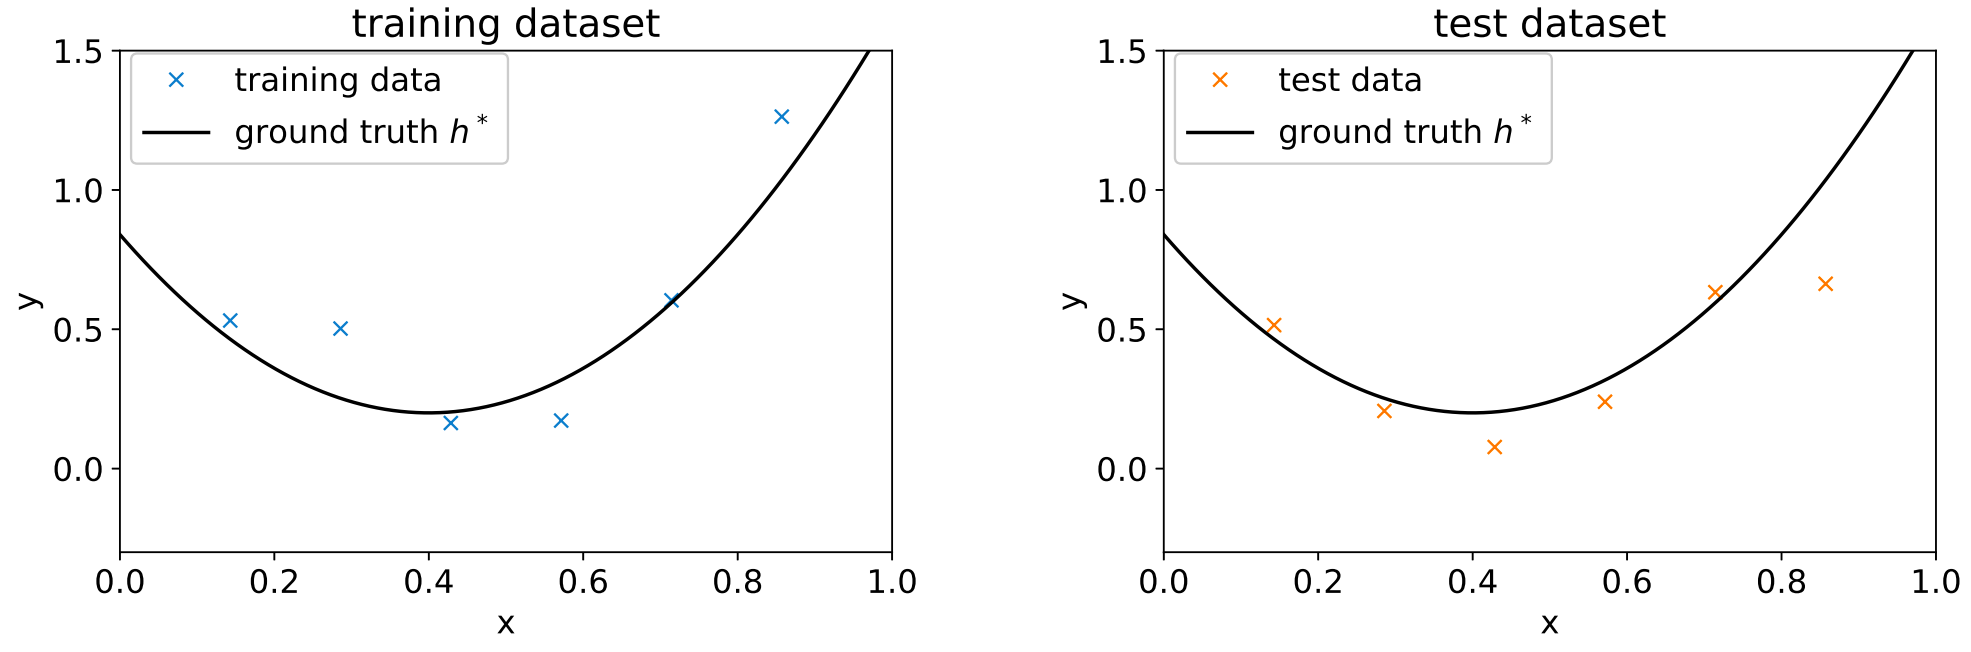
\includegraphics[width=0.8\linewidth]{figs/fitting_gt.png}
    \caption{用于本节的一个训练数据集和测试数据集的示例}
    \label{fig:8.1}
\end{figure}

作为说明性示例,考虑图 \ref{fig:8.1} 所示的训练数据集和测试数据集。训练输入 $x^{(i)}$ 是随机选择的,输出 $y^{(i)}$ 由 $y^{(i)} = h^*(x^{(i)}) + \xi^{(i)}$ 生成,其中函数 $h^*(\cdot)$ 是一个二次函数,在图 \ref{fig:8.1} 中以实线显示,而 $\xi^{(i)}$ 是假定从 $\sim N(0, \sigma^2)$ 生成的观测噪声。测试样本 $(x, y)$ 也有相同的输入-输出关系 $y = h^*(x) + \xi$,其中 $\xi \sim N(0, \sigma^2)$。预测噪声 $\xi$ 是不可能的,因此本质上我们的目标是恢复函数 $h^*(\cdot)$。

将考虑学习各种类型模型的测试误差。在讨论线性回归时,讨论了拟合“简单”模型,例如线性模型 $y = \theta_0 + \theta_1 x$,还是更“复杂”的模型,例如多项式模型 $y = \theta_0 + \theta_1 x + \dots + \theta_5 x^5$ 的问题。

从拟合线性模型开始,如图 \ref{fig:8.2} 所示。即使在训练数据集上,最佳拟合线性模型也无法准确预测 $y$ 与 $x$ 的关系,更不用说在测试数据集上了。这是因为 $y$ 和 $x$ 之间的真实关系不是线性的——任何线性模型都远离真实函数 $h^*(\cdot)$。因此,训练误差很大,这是\textit{欠拟合}的典型情况。

\begin{figure}[H]
    \centering
    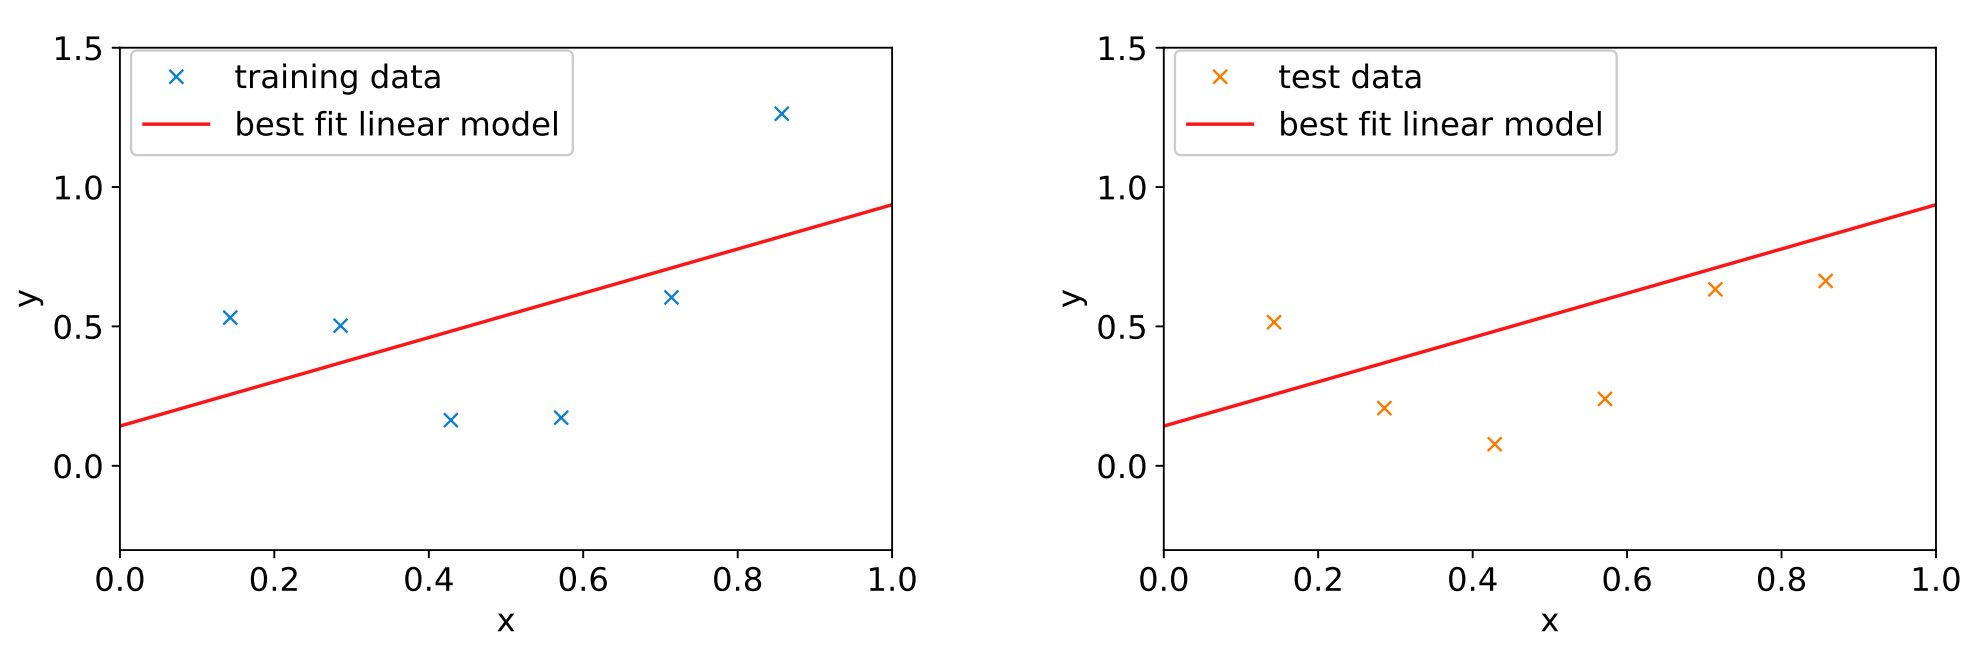
\includegraphics[width=0.8\linewidth]{figs/fitting_linear.png}
    \caption{最好的线性拟合模型也有着巨大的训练和测试误差。}
    \label{fig:8.2}
\end{figure}

\begin{figure}[H]
    \centering
    \begin{minipage}{0.475\linewidth}
        \centering
        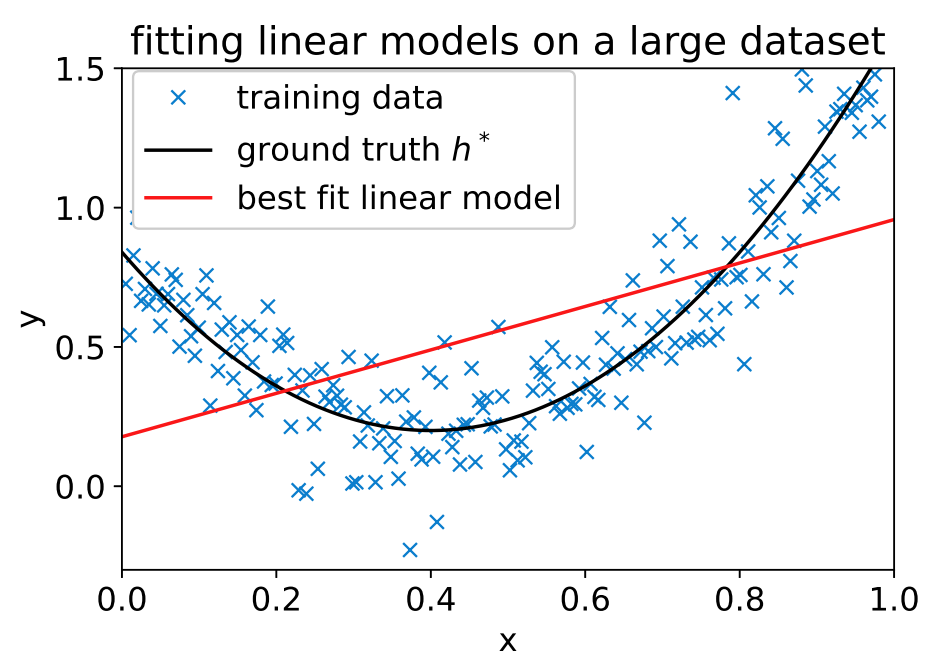
\includegraphics[{width=0.85\linewidth}]{figs/fitting_large.png}
        \caption{最好的线性拟合模型在超大训练集上也有着巨大的训练误差。}
        \label{fig:8.3}
    \end{minipage}\quad
    \begin{minipage}{0.475\linewidth}
        \centering
        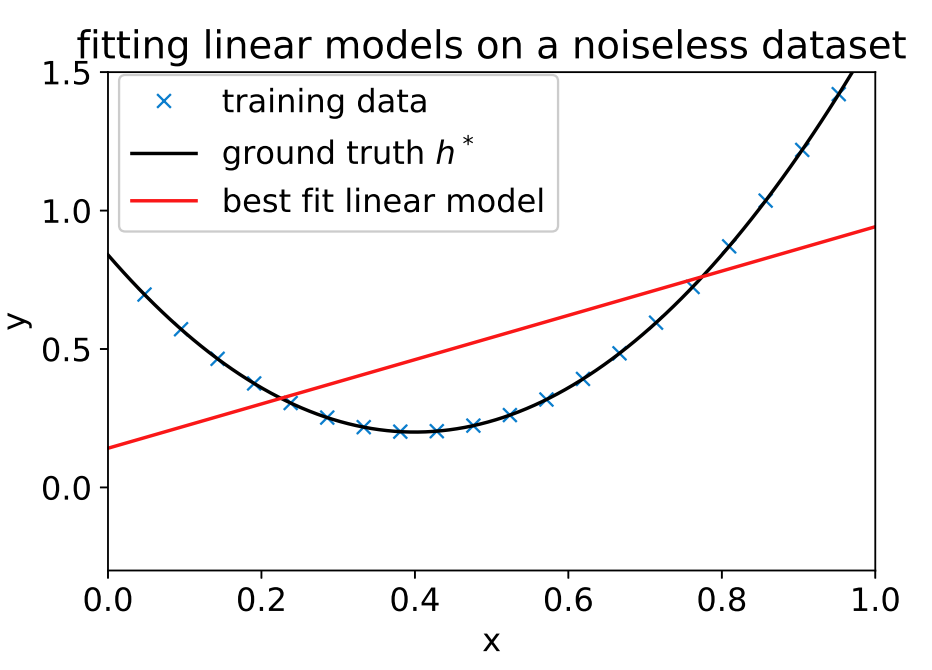
\includegraphics[width=0.85\linewidth]{figs/fitting_noiseless.png}
        \caption{最好的线性拟合模型在没有噪声的训练集上也有着巨大的训练和测试误差。}
        \label{fig:8.4}
    \end{minipage}
\end{figure}

这个问题不能通过增加训练样本来缓解——即使有非常大量的,甚至无限的训练样本,最佳拟合的线性模型仍然不准确,并且无法捕捉数据的结构(图 \ref{fig:8.3})。即使训练数据中不存在噪声,问题仍然存在(图 \ref{fig:8.4})。因此,这里的根本瓶颈在于线性模型族无法捕捉数据中的结构——线性模型无法表示真实的二次函数 $h^*$——而不是缺乏数据。非正式地,我们将模型的\textbf{偏差 (bias)} 定义为即使我们将其拟合到非常大(例如,无限大)的训练数据集时的测试误差。因此,在这种情况下,线性模型具有较大的偏差,并且欠拟合(即无法捕捉数据所表现出的结构)。

接下来,我们将一个 5 次多项式拟合到数据。图 \ref{fig:8.5} 表明它也未能学习到一个好的模型。然而,其失败模式与线性模型的情况不同。具体来说,尽管学习到的 5 次多项式在预测训练样本的 $y^{(i)}$ 与 $x^{(i)}$ 时表现非常好,但在测试样本上效果不佳(图 \ref{fig:8.5})。换句话说,从训练集学习到的模型无法很好地\textit{泛化 (generalize)} 到其他测试样本——测试误差很高。与线性模型的行为相反,5 次多项式的偏差较小——如果我们将 5 次多项式拟合到非常大的数据集,得到的模型将接近二次函数并且也很准确(图 \ref{fig:8.6})。这是因为 5 次多项式族包含所有二次函数(将 $\theta_5 = \theta_4 = \theta_3 = 0$ 设置为零即可得到二次函数),因此,原则上 5 次多项式能够捕捉数据的结构。

\begin{figure}[H]
    \centering
    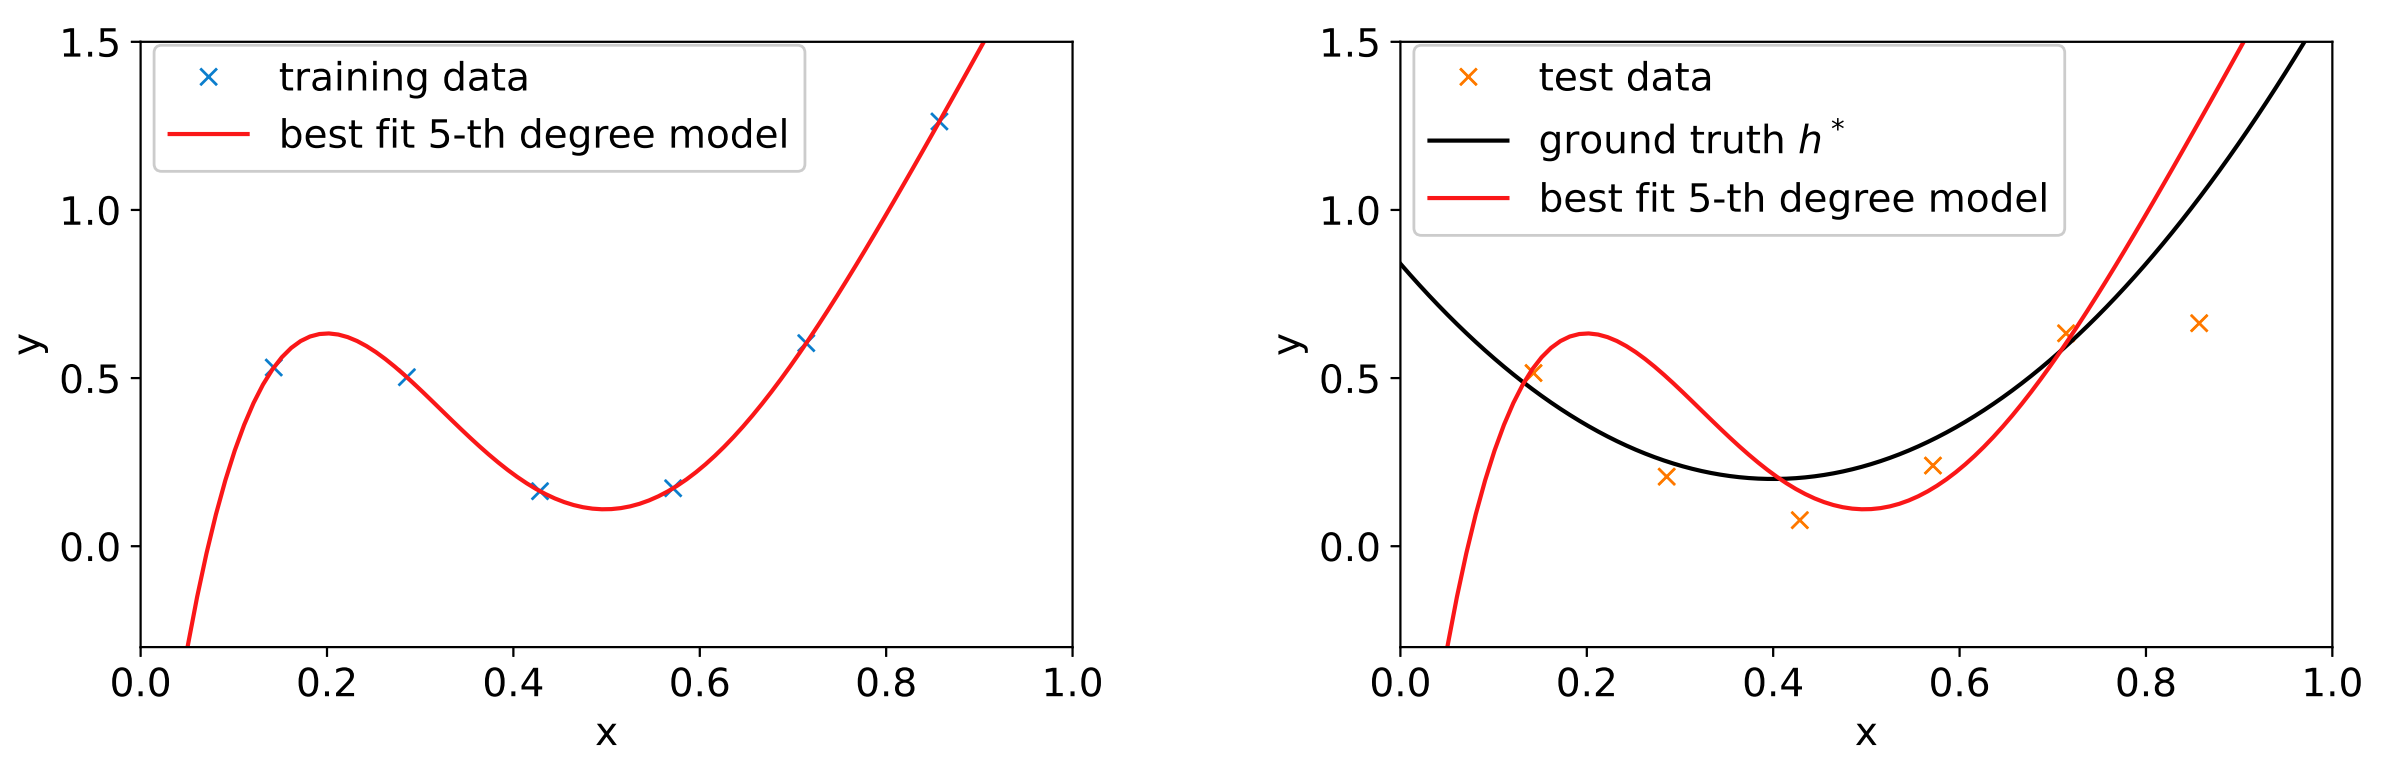
\includegraphics[width=0.8\linewidth]{figs/fitting_5th.png}
    \caption{最佳的 5 次多项式拟合模型训练误差为零,但测试误差仍然很大,并且未能恢复真实情况。这是经典的过拟合情形。}
    \label{fig:8.5}
\end{figure}

\begin{figure}[H]
    \centering
    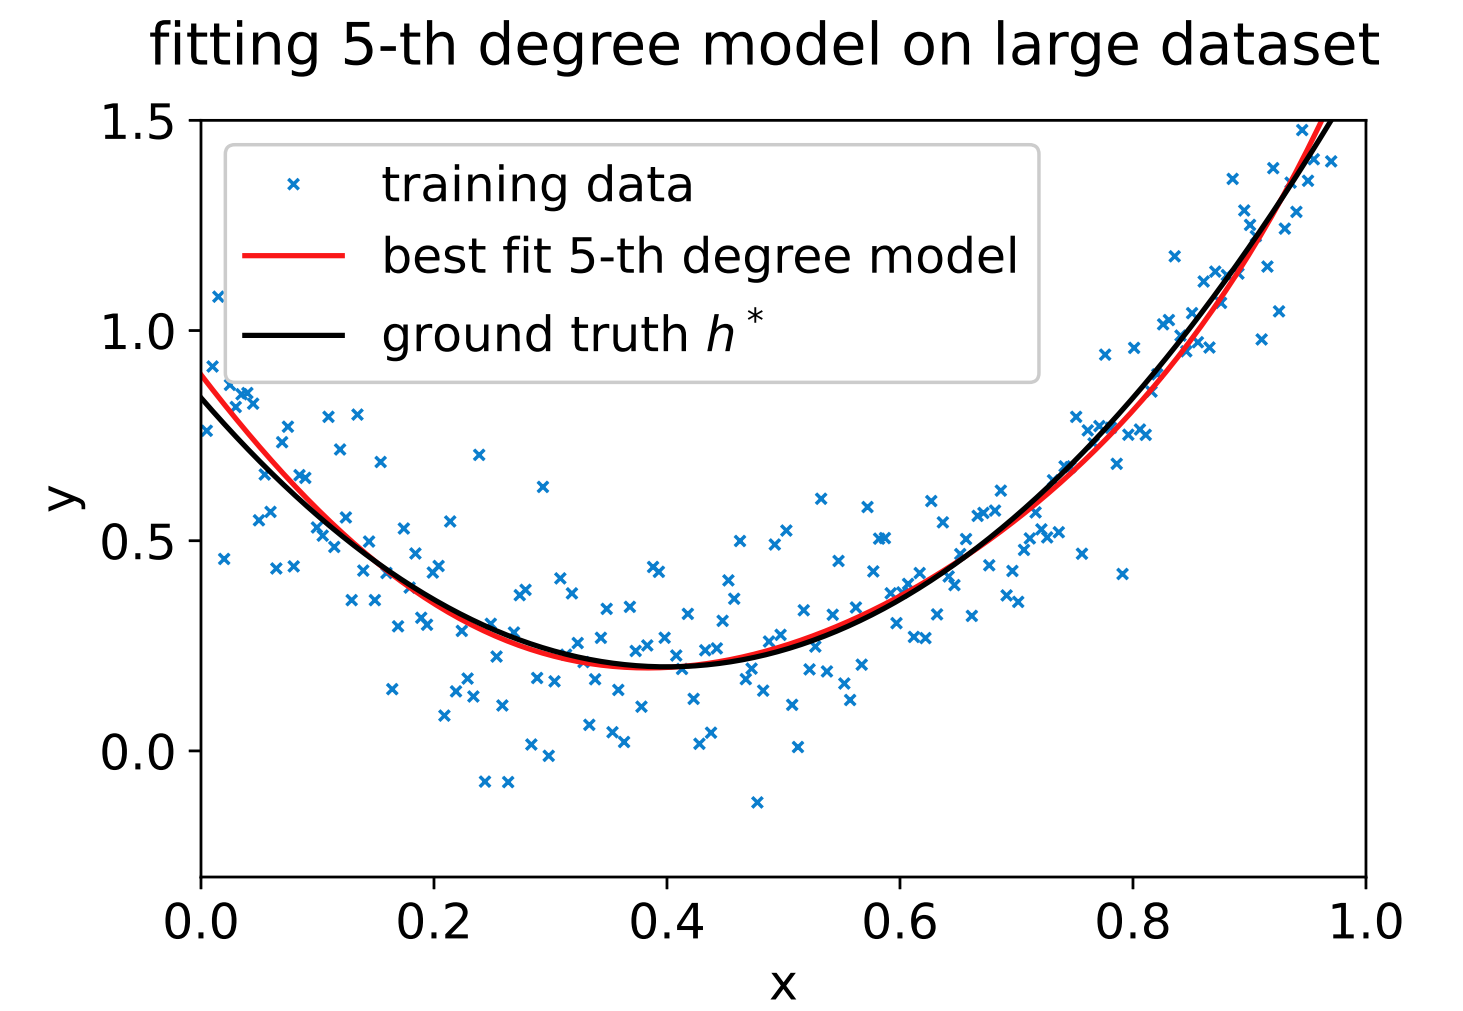
\includegraphics[width=0.5\linewidth]{figs/fitting_5th_large.png}
    \caption{在大型数据集上拟合的最佳 5 次多项式几乎恢复了真实情况——这表明图 \ref{fig:8.5} 中的问题是方差(或数据不足)而不是偏差。}
    \label{fig:8.6}
\end{figure}

拟合 5 次多项式的失败可以用测试误差的另一个组成部分来解释,称为模型拟合过程的\textbf{方差 (variance)}。具体来说,如图 \ref{fig:8.7} 所示,在拟合 5 次多项式时,存在很大的风险,即我们拟合了数据中恰好存在于我们\textit{小而有限 (small, finite)} 的训练集中的模式,但这些模式并不能反映 $x$ 和 $y$ 之间关系的更广泛模式。训练集中的这些“虚假”模式(大部分)是由于观测噪声 $\xi^{(i)}$ 引起的,拟合这些虚假模式会导致模型具有较大的测试误差。在这种情况下,我们称模型具有较大的方差。

\begin{figure}[H]
    \centering
    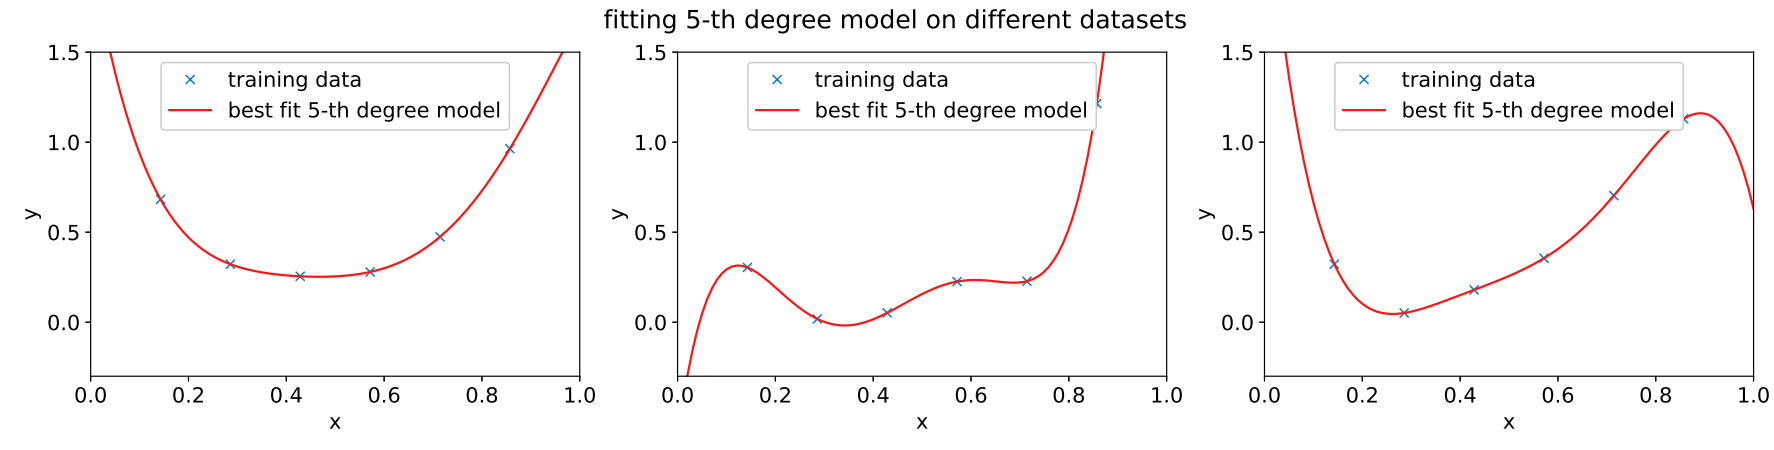
\includegraphics[width=0.95\linewidth]{figs/fitting_5th_different.png}
    \caption{在三个从同一分布产生的不同数据集上拟合的最佳 5 次多项式表现出极大不同,揭示其存在的巨大方差。}
    \label{fig:8.7}
\end{figure}

方差可以直观地(以及数学上证明,如第 \ref{sec:8.1.1} 节所示)通过在多个不同的训练数据集(从相同的潜在分布中抽取)上学习到的模型之间的变化量来表征。“虚假模式”是特定于特定数据集中的噪声(和输入)的随机性,因此在多个训练数据集之间是不同的。因此,对多个数据集的“虚假模式”过拟合应该会导致非常不同的模型。实际上,如图 \ref{fig:8.7} 所示,在三个不同训练数据集上学习到的模型差异很大,对每个数据集的“虚假模式”都存在过拟合。通常,偏差和方差之间存在权衡。如果我们的模型过于“简单”且参数很少,那么它可能具有较大的偏差(但方差较小),并且通常会遭受欠拟合。如果它过于“复杂”且参数很多,那么它可能遭受较大的方差(但偏差较小),因此会过拟合。图 \ref{fig:8.8} 展示了偏差和方差之间典型的权衡关系。

\begin{figure}[H]
    \centering
    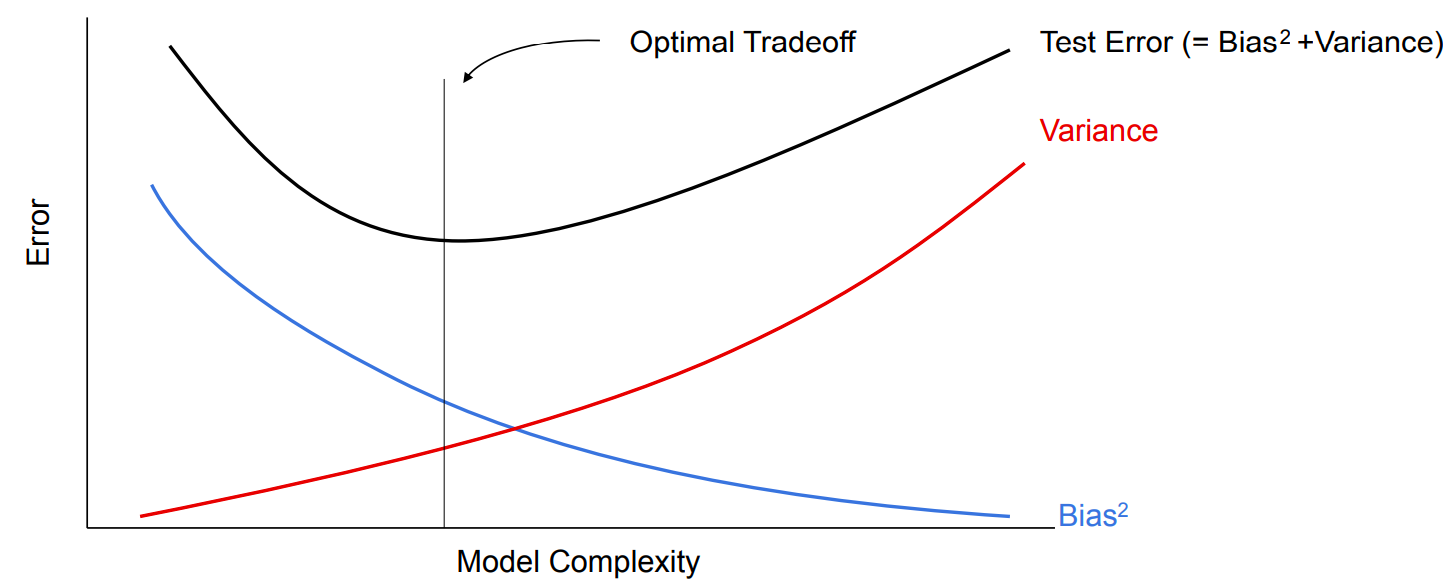
\includegraphics[width=0.9\linewidth]{figs/bias-variance_tradeoff.png}
    \caption{典型的偏差-方差权衡示意图。}
    \label{fig:8.8}
\end{figure}

正如我们将在第 \ref{sec:8.1.1} 节中正式看到的,测试误差可以分解为偏差和方差之和。这意味着随着模型复杂度的增加,测试误差将呈现凸曲线,在实践中我们应该调整模型复杂度以达到最佳权衡。例如,在上面的例子中,拟合二次函数比拟合一次或五次多项式效果更好,如图 \ref{fig:8.9} 所示。

\begin{figure}[H]
    \centering
    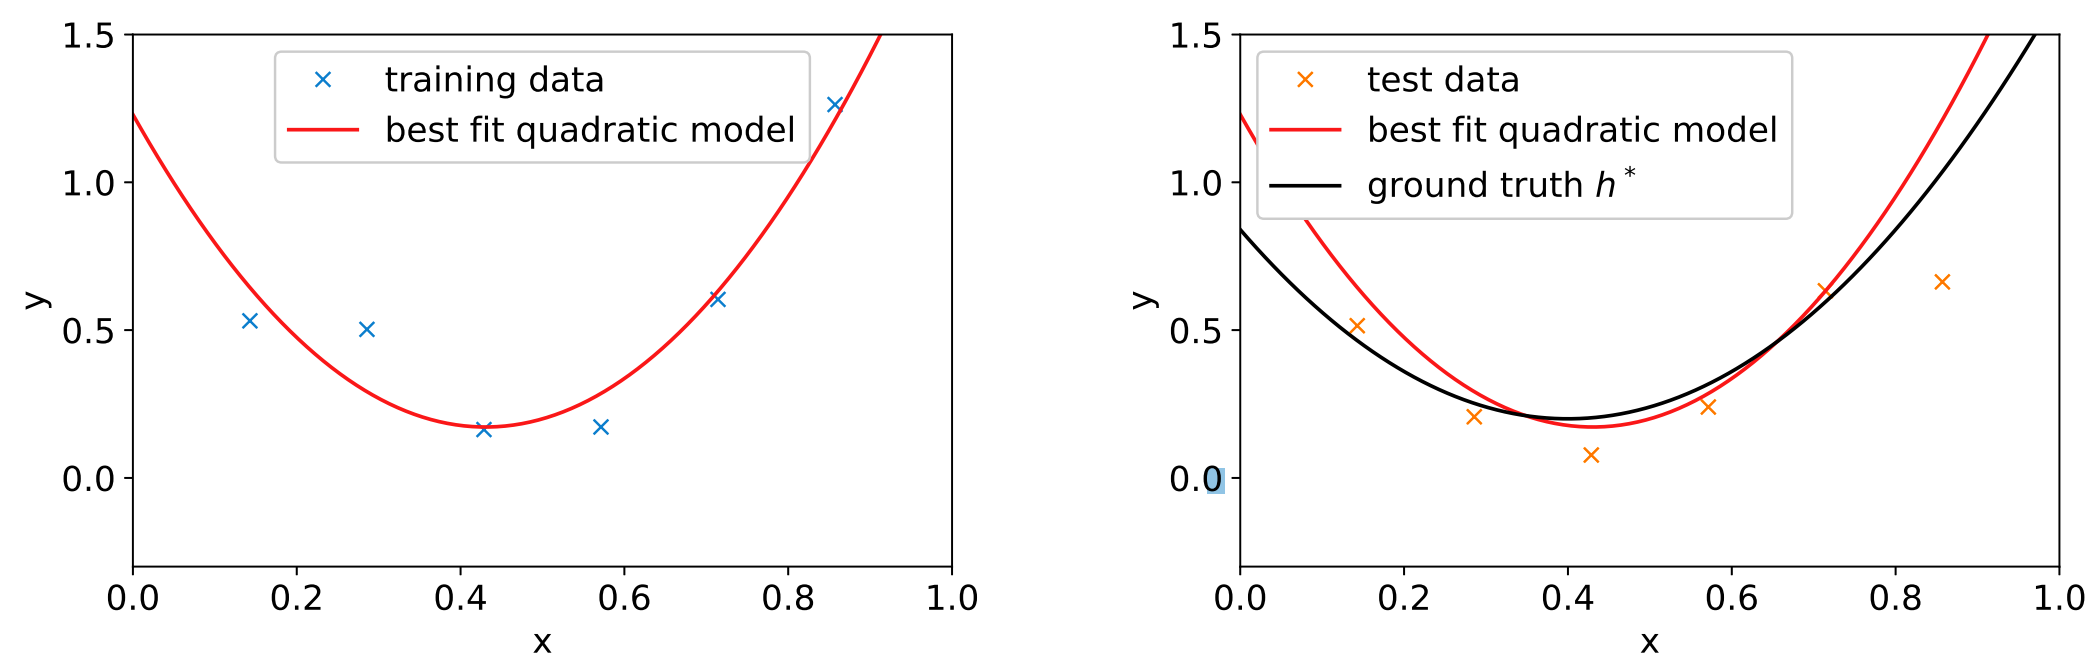
\includegraphics[width=0.8\linewidth]{figs/fitting_quadratic.png}
    \caption{最佳的二次拟合模型的训练误差和测试误差都很小,因为二次模型达到了良好的偏差-方差权衡。}
    \label{fig:8.9}
\end{figure}

有趣的是,偏差-方差权衡曲线或测试误差曲线并不普遍遵循图 \ref{fig:8.8} 中的形状,至少当模型复杂度仅通过参数数量衡量时并非如此。(我们将在 \ref{sec:8.2} 节中讨论所谓的双下降现象。)尽管如此,偏差-方差权衡原理在分析和预测测试误差的行为时,可能仍然是首选方法。

\subsection{(对于回归问题的)数学分解}\label{sec:8.1.1}

为了形式化回归问题的偏差-方差权衡,我们考虑如下设置(这是 \ref{sec:8.1} 节开头段落的扩展)
\begin{itemize}
    \item 抽取一个训练数据集 $S = \{x^{(i)}, y^{(i)}\}_{i=1}^n$,其中 $y^{(i)} = h^*(x^{(i)}) + \xi^{(i)}$ 且 $\xi^{(i)} \in N(0, \sigma^2)$。
    \item 在数据集 $S$ 上训练一个模型,记为 $\hat{h}_S$。
    \item 取一个测试样本 $(x, y)$,使得 $y = h^*(x) + \xi$ 且 $\xi \sim N(0, \sigma^2)$,并测量测试误差的期望(在随机抽取的训练集 $S$ 和随机的 $\xi$ 上进行平均)\footnote{为简单起见,这里测试输入 $x$ 被视为固定,但在对 $x$ 进行平均时,同样的思想仍然成立。}\footnote{期望符号下的下标是为了强调在期望运算中被视为随机的变量。}。
\end{itemize}
\begin{equation}
    \text{MSE}(x) = \mathbb{E}_{S, \xi}[(y - \hat{h}_S(x))^2] \label{eq:8.2}
\end{equation}

我们将把 MSE 分解为偏差项和方差项。我们从一个简单的数学工具开始,该工具将在下面使用两次。

\begin{claim}\label{claim:8.1.1}
    假设 $A$ 和 $B$ 是两个独立的实随机变量,且 $\mathbb{E}[A] = 0$。则 $\mathbb{E}[(A + B)^2] = \mathbb{E}[A^2] + \mathbb{E}[B^2]$。\\
    推论:因为随机变量 $A$ 与常数 $c$ 独立,当 $\mathbb{E}[A] = 0$ 时,我们有 $\mathbb{E}[(A+c)^2] = \mathbb{E}[A^2] + c^2$。
\end{claim}

断言的证明通过展开平方项得出:$\mathbb{E}[(A + B)^2] = \mathbb{E}[A^2 + B^2 + 2AB] = \mathbb{E}[A^2] + \mathbb{E}[B^2] + 2\mathbb{E}[AB] = \mathbb{E}[A^2] + \mathbb{E}[B^2]$。这里我们使用了独立性来证明 $\mathbb{E}[AB] = \mathbb{E}[A]\mathbb{E}[B] = 0$。
使用断言 \ref{claim:8.1.1},令 $A = \xi$ 且 $B = h^*(x) - \hat{h}_S(x)$,我们有
\begin{align}
    \text{MSE}(x) = \mathbb{E}[(y - \hat{h}_S(x))^2] &= \mathbb{E}[(\xi + (h^*(x) - \hat{h}_S(x)))^2] \label{eq:8.3} \\
    &= \mathbb{E}[\xi^2] + \mathbb{E}[(h^*(x) - \hat{h}_S(x))^2] \quad (\text{根据断言 \ref{claim:8.1.1}})  \nonumber\\
    &= \sigma^2 + \mathbb{E}[(h^*(x) - \hat{h}_S(x))^2] \label{eq:8.4}
\end{align}

然后,我们定义 $h_{\text{avg}}(x) = \mathbb{E}_S[\hat{h}_S(x)]$ 为“平均模型”——通过抽取无限多个数据集,并在其上进行训练,然后对它们在 $x$ 上的预测进行平均而获得的模型。注意,$h_{\text{avg}}$ 是一个用于分析目的的假设模型,它在现实中无法获得(因为我们无法拥有无限多个数据集)。结果表明,对于许多情况,$h_{\text{avg}}$(近似)等于在具有无限样本的单个数据集上训练得到的模型。因此,我们也可以直观地解释 $h_{\text{avg}}$,这与我们在上一小节中对偏差的直观定义一致。

我们可以通过令 $c = h^*(x) - h_{\text{avg}}(x)$(这是一个不依赖于 $S$ 选择的常数)和 $A = h_{\text{avg}}(x) - \hat{h}_S(x)$ 来进一步分解 $\text{MSE}(x)$,这符合断言 \ref{claim:8.1.1} 的推论:

\begin{align}
    \text{MSE}(x) &= \sigma^2 + \mathbb{E}[(h^*(x) - \hat{h}_S(x))^2] \label{eq:8.5} \\
    &= \sigma^2 + \mathbb{E}[(h^*(x) - h_{\text{avg}}(x) + h_{\text{avg}}(x) - \hat{h}S(x))^2] \label{eq:8.6} \\
    &= \underbrace{\sigma^2}_{\text{不可避免}} + \underbrace{(h^*(x) - h_{\text{avg}}(x))^2}_{\text{偏差}^2} + \underbrace{\text{var}(\hat{h}S(x))}_{\text{方差}} \label{eq:8.7}
\end{align}
我们将第二项称为偏差(平方),第三项称为方差。如前所述,偏差捕捉了由于模型表达能力不足而引入的误差部分。回想一下,$h_{\text{avg}}$ 可以被认为是即使在无限数据下学习到的最佳可能模型。因此,偏差并非根本上由数据不足引起,而是由模型族本身无法很好地近似 $h^*$ 造成的。例如,在图 \ref{fig:8.2} 所示的例子中,由于任何线性模型都无法近似真实的二次函数 $h^*$,因此 $h_{\text{avg}}$ 也不能,从而偏差项很大。
方差项捕捉了有限数据集的随机性如何引入学习模型中的误差。它衡量了学习模型对数据集中随机性的敏感度。随着数据集大小的增加,方差通常会减小。
对于第一项 $\sigma^2$,我们无能为力,因为根据定义,我们无法预测噪声 $\xi$。
最后,我们注意到,分类问题的偏差-方差分解远不如回归问题清晰。已经有一些提案,但对于什么是“正确”和/或最有用的形式还没有达成一致。


\section{双下降现象}\label{sec:8.2}

\subsection*{模型层面的双下降现象}

最近的研究表明,在包括线性模型和深度神经网络在内的一系列机器学习模型中,测试误差会呈现出一种“双下降”现象\footnote{该现象的发现可能可以追溯到 \cite{opper1995statistical,opper2001learning},最近由 \cite{belkin2020two,hastie2022surprises} 推广。}。正如 \ref{sec:8.1} 节中所讨论的传统观点是,随着模型复杂度的增加,测试误差先下降然后上升,如图 \ref{fig:8.8} 所示。然而,在许多情况下,我们经验性地观察到测试误差可以有第二次下降——它先下降,然后在大到足以很好地拟合所有训练数据时达到峰值附近,然后在所谓的过参数化区域再次下降,其中参数数量大于数据点数量。图 \ref{fig:8.10} 展示了测试误差随模型复杂度(由参数数量衡量)变化的典型曲线。在某种程度上,过参数化区域的第二次下降被认为是机器学习领域的新发现——部分原因是轻度正则化的过参数化模型在深度学习时代得到了广泛应用。这种现象的一个实际意义是,不应回避扩大模型规模和尝试过参数化模型,因为测试误差很可能再次下降到比之前的最低点更低的水平。实际上,在许多情况下,更大的过参数化模型总是能带来更好的测试性能(这意味着第二次下降之后不会出现第二次上升)。

\begin{figure}[H]
    \centering
    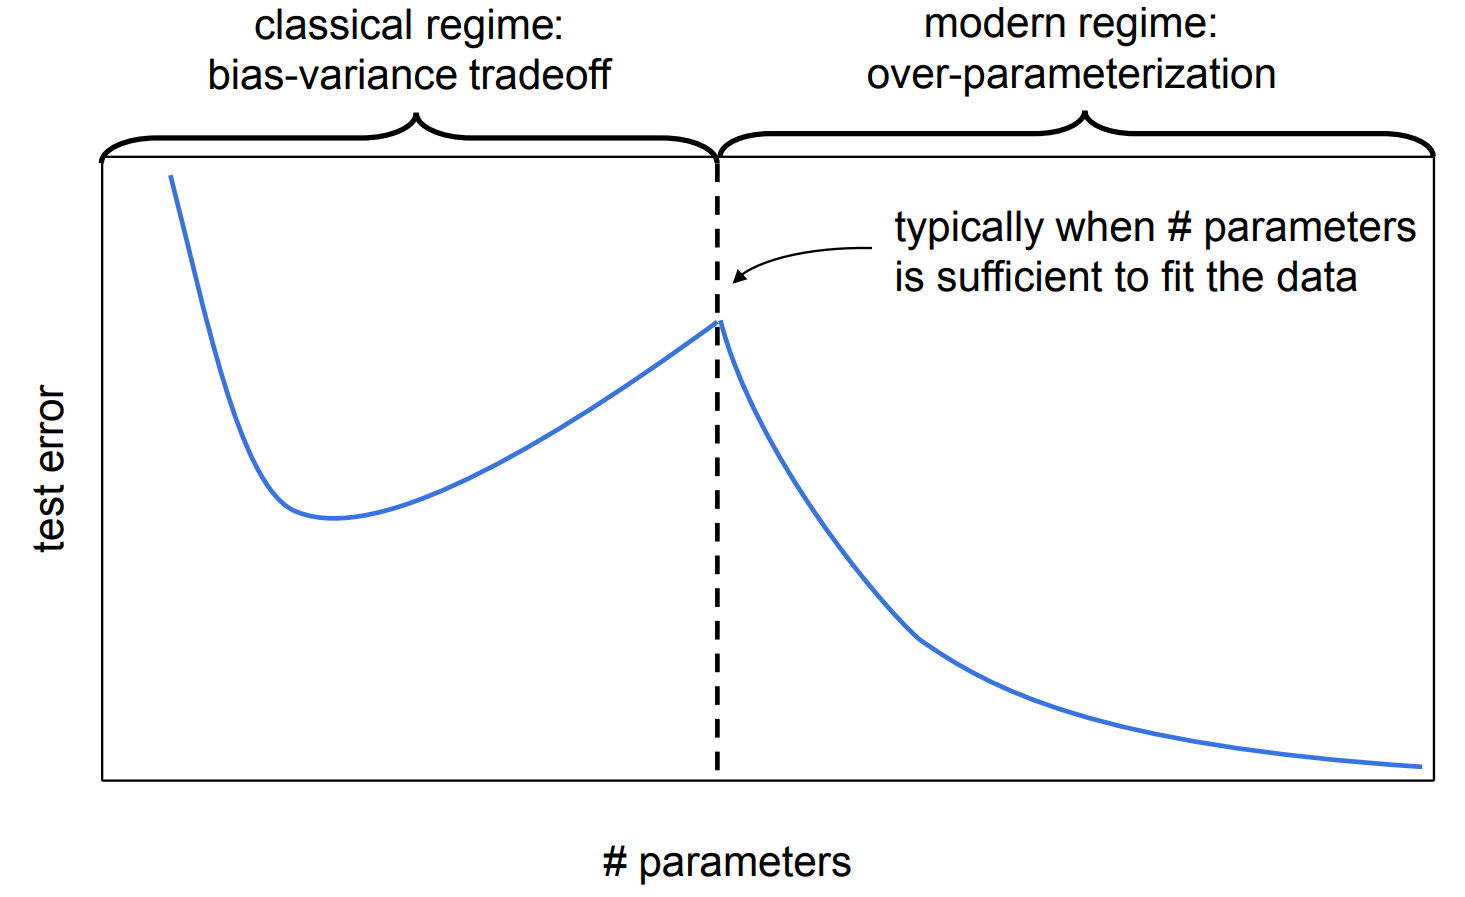
\includegraphics[width=0.8\linewidth]{figs/double_descent.png}
    \caption{典型的模型层面双下降现象。随着参数数量的增加,当参数数量小于训练数据时,测试误差先下降。然后在过参数化区域,测试误差再次下降。}
    \label{fig:8.10}
\end{figure}

\subsection*{样本层面的双下降现象}

从先验知识来看,我们期望更多的训练样本总是能带来更小的测试误差——更多的样本为算法提供了更严格的信息来学习。然而,最近的研究 [\cite{nakkiran2019more}] 观察到,随着样本数量的增加,测试误差并非单调递减。相反,如图 \ref{fig:8.11} 所示,测试误差先下降,然后在样本数量(记为 $n$)与参数数量(记为 $d$)接近时增加并达到峰值,然后再次下降。我们将此称为样本层面的双下降现象。在某种程度上,样本层面的双下降和模型层面的双下降本质上描述的是类似的现象——测试误差在 $n \approx d$ 时达到峰值。

\begin{figure}[H]
    \centering
    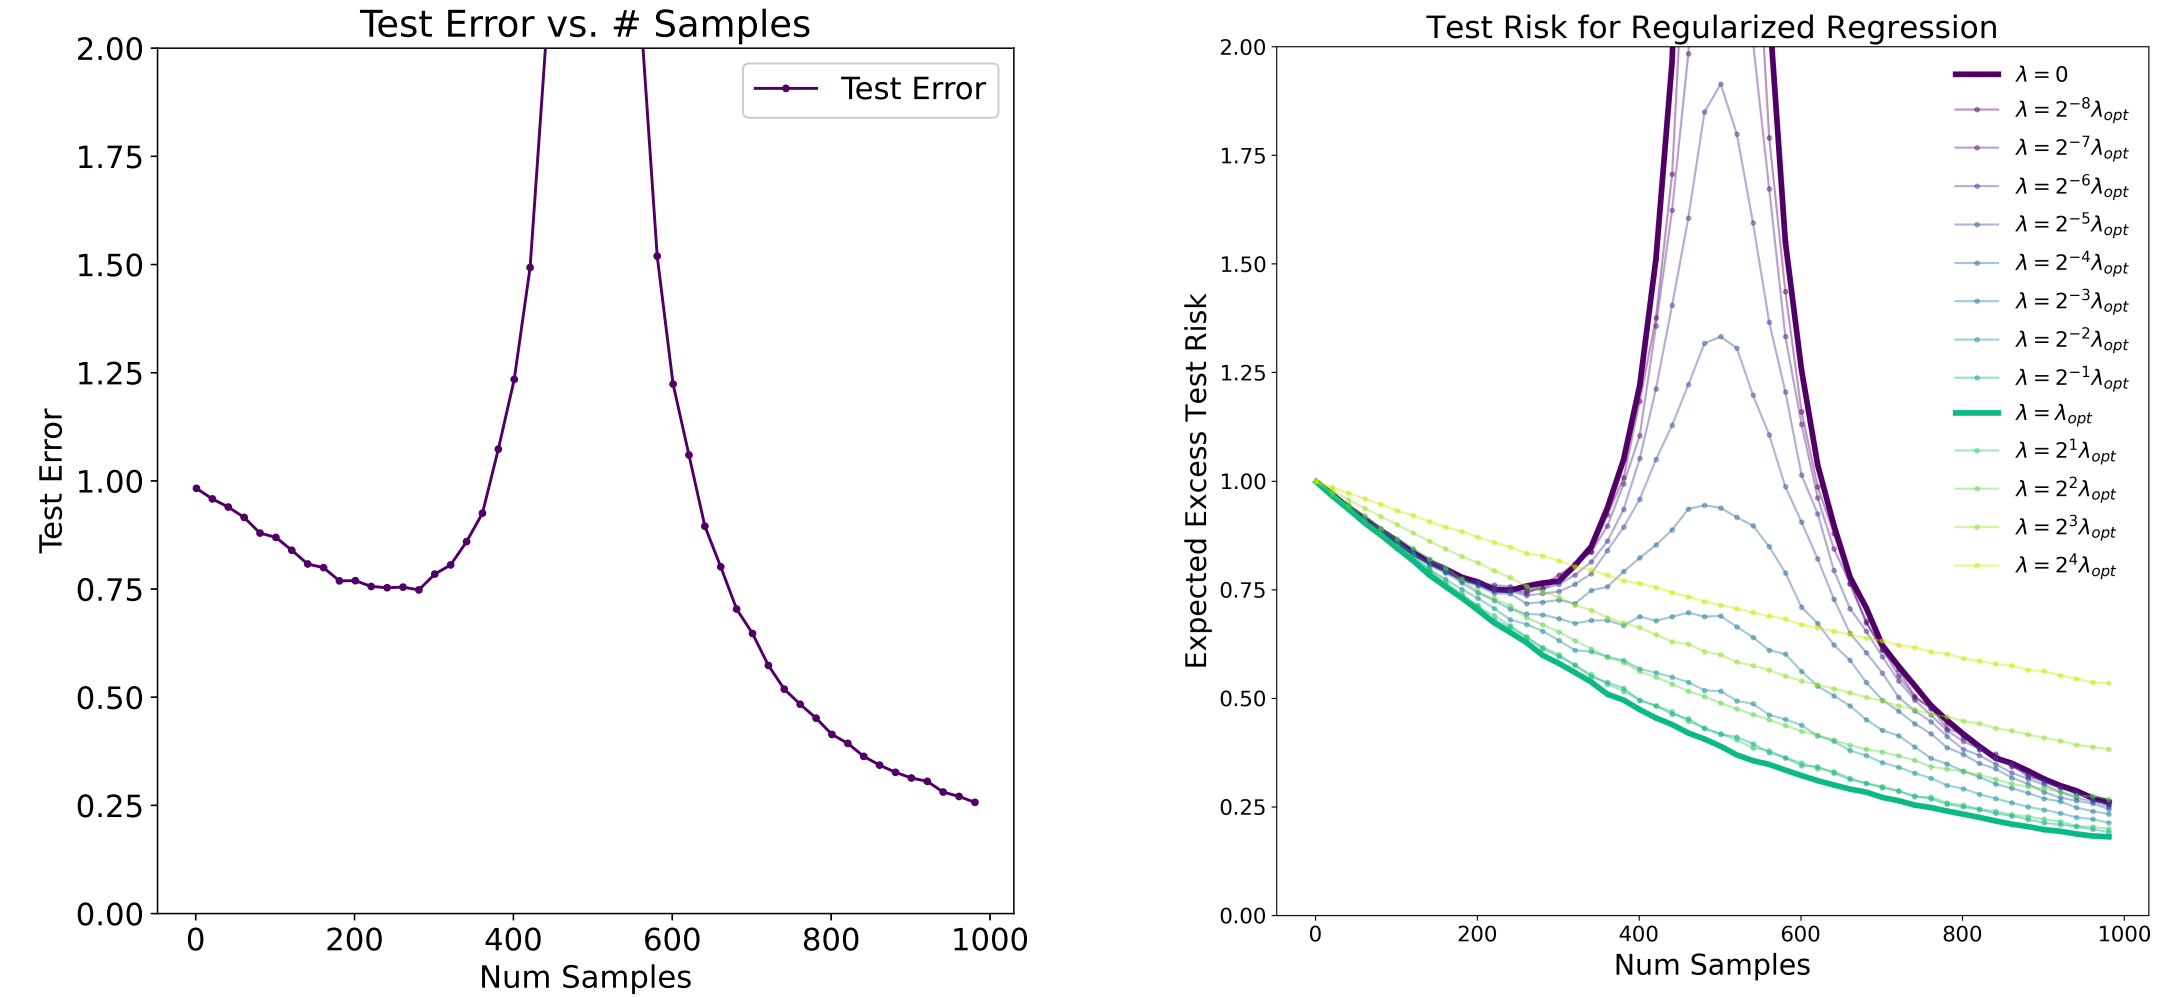
\includegraphics[width=0.9\linewidth]{figs/sample_double_descent.png}
    \caption{\textbf{左:}线性模型在样本层面的双下降现象。\textbf{右:}不同正则化强度下线性模型在样本层面的双下降现象。 使用最优正则化参数(对每个 $n$ 都调到最优,以绿色实线显示)缓解双下降。 \textbf{设置:}$(x, y)$ 的数据分布为 $x \sim \mathcal{N}(0, I_d)$ 且 $y \sim x^\top \beta + \mathcal{N}(0, \sigma^2)$,其中 $d = 500$, $\sigma = 0.5$ 且 $\|\beta\|_2 = 1$.\protect\footnotemark}
    \label{fig:8.11}
\end{figure}
\footnotetext[8]{此图依照 \cite{nakkiran2020optimal} 的图 1 复现,类似的现象也可以在 \cite{hastie2022surprises,mei2022generalization} 中观察到。}

\subsection*{解释和缓解策略}

样本层面的双下降,特别是测试误差在 $n \approx d$ 处的峰值,表明在这些实验中评估的现有训练算法在 $n \approx d$ 时远非最优。我们可以通过丢弃一些样本,使用较小的样本量运行算法来避免峰值。换句话说,原则上存在其他算法可以在 $n \approx d$ 时实现更小的测试误差,但这些实验中评估的算法未能做到。学习过程的次优性似乎是样本层面和模型层面双下降峰值的罪魁祸首。
实际上,通过最优调整的正则化(将在第 \ref{chapter:9} 章中更详细讨论),在 $n \approx d$ 区域的测试误差可以显著改善,并且模型层面和样本层面的双下降现象都得到了缓解。参见图 \ref{fig:8.11}。
上述直觉只解释了模型层面和样本层面双下降的峰值,但没有解释模型层面双下降的第二次下降——为什么过参数化模型能够很好地泛化。对过参数化模型的理论理解是一个活跃的研究领域,最近取得了许多进展。一个典型的解释是,常用的优化器(如梯度下降)提供了隐式正则化效应(将在第 9.2 节中更详细讨论)。换句话说,即使在过参数化区域且使用了非正则化的损失函数,模型仍然隐式地进行了正则化,因此表现出比拟合数据的任意解更好的测试性能。例如,对于线性模型,当 $n \ll d$ 时,使用零初始化进行梯度下降的优化器会找到拟合数据的\textit{最小范数 (minimum norm)} 解(而不是拟合数据的任意解),而最小范数正则化器对于过参数化区域来说是一个足够好的正则化器(但在 $n \approx d$ 时不是一个好的正则化器,导致测试误差达到峰值)。

\begin{figure}[H]
    \centering
    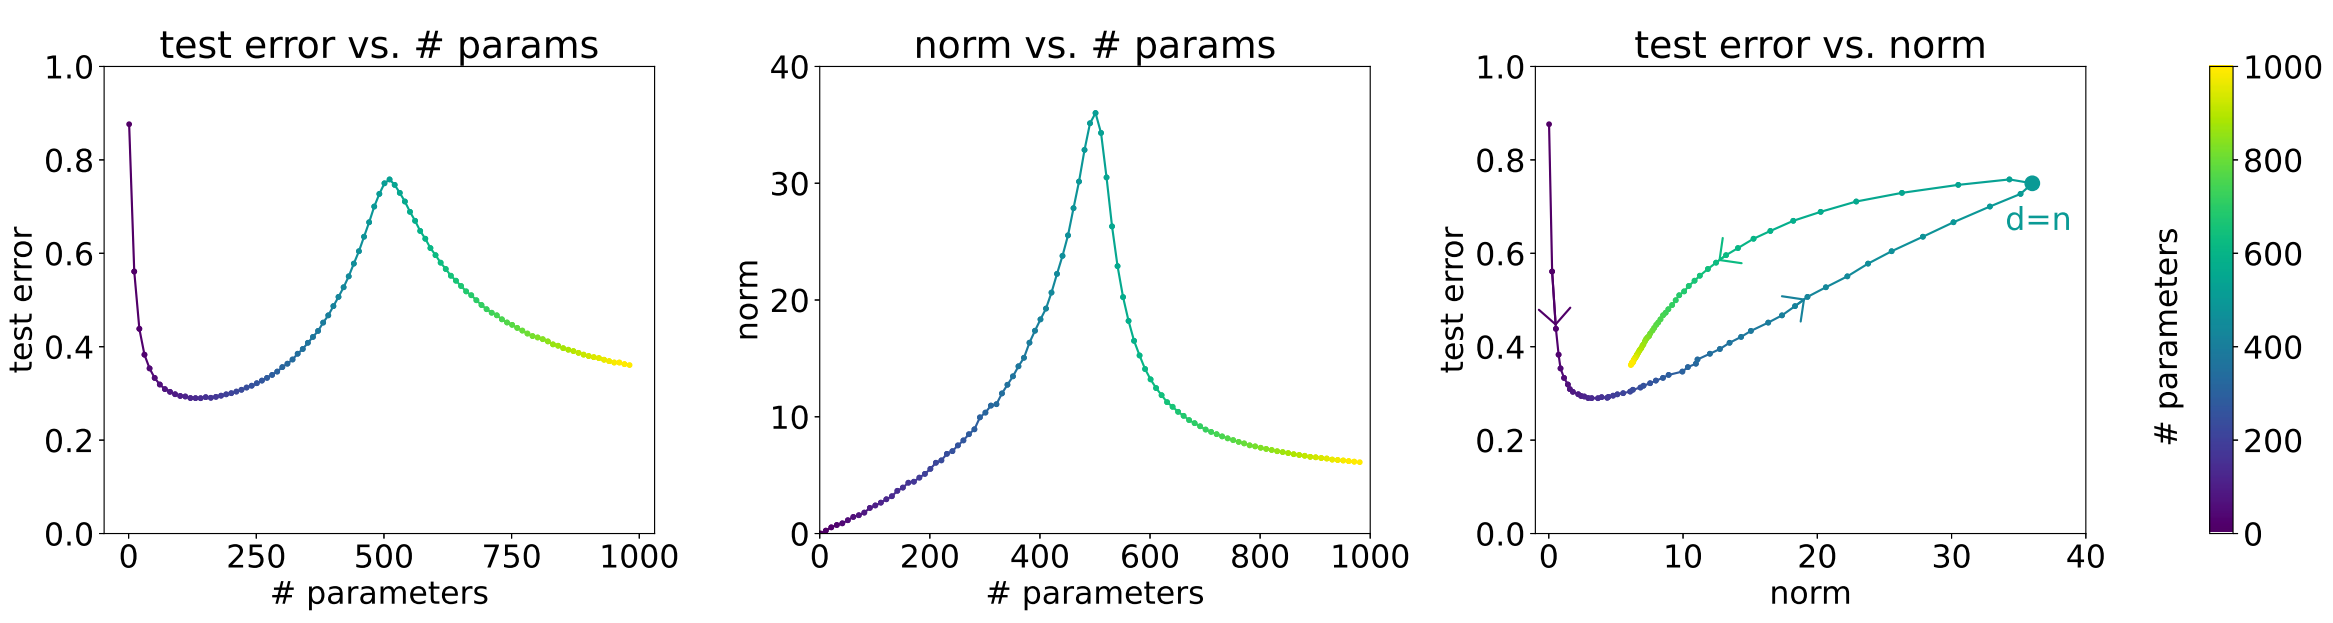
\includegraphics[width=1.0\linewidth]{figs/double_descent_norm.png}
    \caption{\textbf{左:}双下降现象,其中模型复杂度用参数数量来衡量。\textbf{中:}学习到的模型的范数在 $n \approx d$ 附近达到峰值。\textbf{右:}测试误差与学习到的模型范数的关系。颜色条表示参数数量,箭头表示模型尺寸增加的方向。它们的关系更接近于传统认知,而不是双下降。 \textbf{设置}:我们考虑一个样本量固定为 $n = 500$ 的线性回归。输入 $x$ 是 Fashion-MNIST 上的随机 ReLU 特征,输出 $y \in \mathbb{R}^{10}$ 是 one-hot 标签。这与 \cite{nakkiran2020optimal} 第 5.2 节中的设置相同。}
    \label{fig:8.12}
\end{figure}

最后,我们还要指出,双下降现象主要在模型的复杂度用参数数量来衡量时被观察到。参数数量是否以及何时是衡量模型复杂度的最佳指标尚不清楚。例如,在许多情况下,模型的范数被用作复杂度度量。如图 \ref{fig:8.12} 右图所示,对于一个特定的线性情况,如果我们绘制测试误差与学习到的模型范数的关系,双下降现象就不再发生。这部分是因为学习到的模型的范数在 $n \approx d$ 附近也达到峰值(参见图 \ref{fig:8.12}(中)或 \cite{belkin2019reconciling}、\cite{mei2022generalization},以及 \cite{james2021introduction} 在第 10.8 节中的讨论)。对于深度神经网络,正确的复杂度度量更加难以捉摸。双下降现象的研究仍是一个活跃的研究课题。

\section{样本复杂度边界 (选读)}\label{sec:8.3}

